
\section{Running Sampler}

\subsection{About Sampler}
 \begin{itemize}
  \item If you are happy with the results of the Bertini\_real decomposition, you may wish to refine the triangulation of the surface or curve. This can be acheived using the \texttt{sampler} program after calling \texttt{bertini\_real}. 
  \item This section will show you how to:
   \begin{enumerate}
   	\item Properly run sampler, with visual examples
   	\item Use the different algorithms to shape curves and surfaces
   	\item Use matlab to better visualize curves and surfaces
   \end{enumerate}
 \end{itemize}  

 \subsection{Curves}
 
 	\subsubsection{Running Sampler (Using an Example)}
 	 In order to show how to properly run sampler, I will be using an example of a curve, going through each step to make sure the basics of sampler are covered.
 		\begin{longtabu} to \textwidth {
    X[1,c]
    X[1,c]}
\hline
\rowfont\bfseries
\textbf{Instructions} & \textbf{Screen Shot} \\
\hline  \\ 
\endfirsthead
\caption[]{\textit{Continued from previous page}}\\
\hline
\textbf{Instructions} & \textbf{Screen Shot} \\
\hline \\
\endhead
\bottomrule \multicolumn{2}{r}{\textit{Continued on next page}} \\
\endfoot
\bottomrule \multicolumn{2}{r}{\textit{}} \\
\endlastfoot
First, choose the curve you wish to produce. (In this case I am choosing the 'eistute\_sphere', which is found in the 'intersections' file which can be found in the 'zoo' file) & 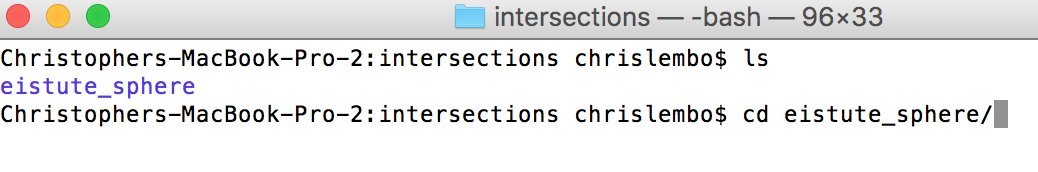
\includegraphics[width=0.4\textwidth]{curvesampler1}  \\  \\  \\
\hline \\
Invoke 'bertini' and 'bertini\_real' & 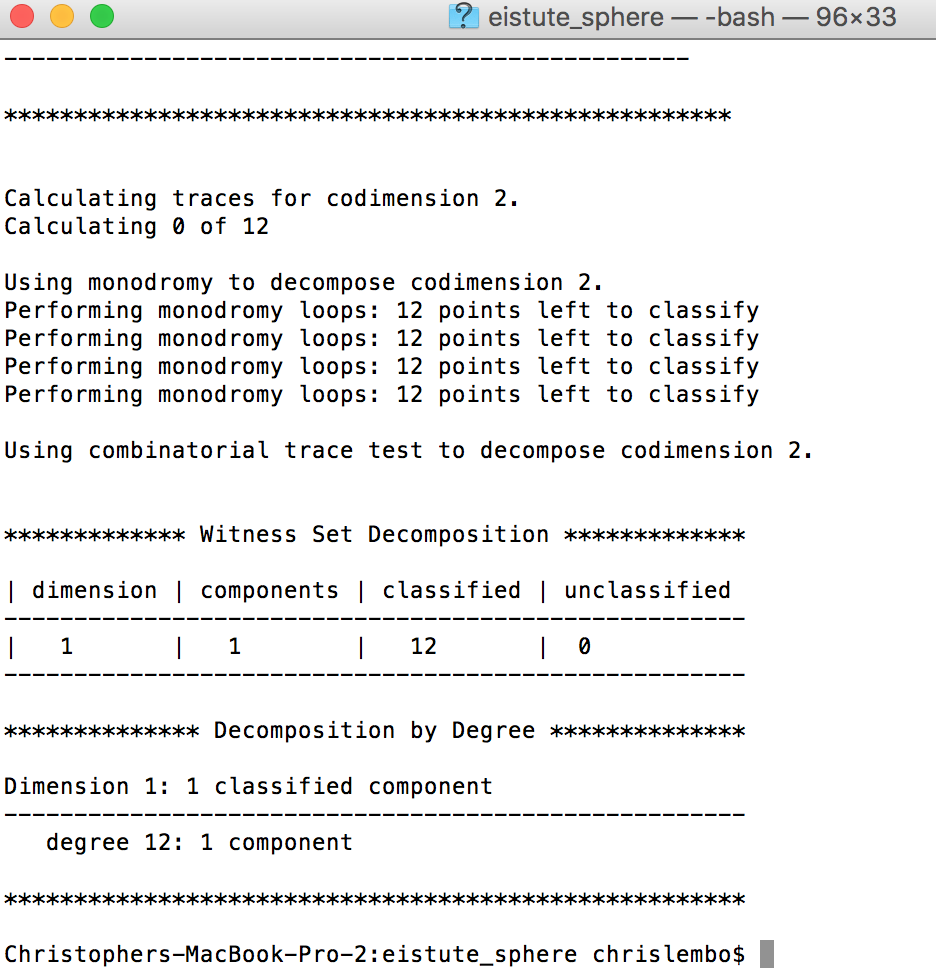
\includegraphics [width=0.4\textwidth]{curvesampler2} \\ \\ \\ 
\hline \\
Invoke 'sampler' & 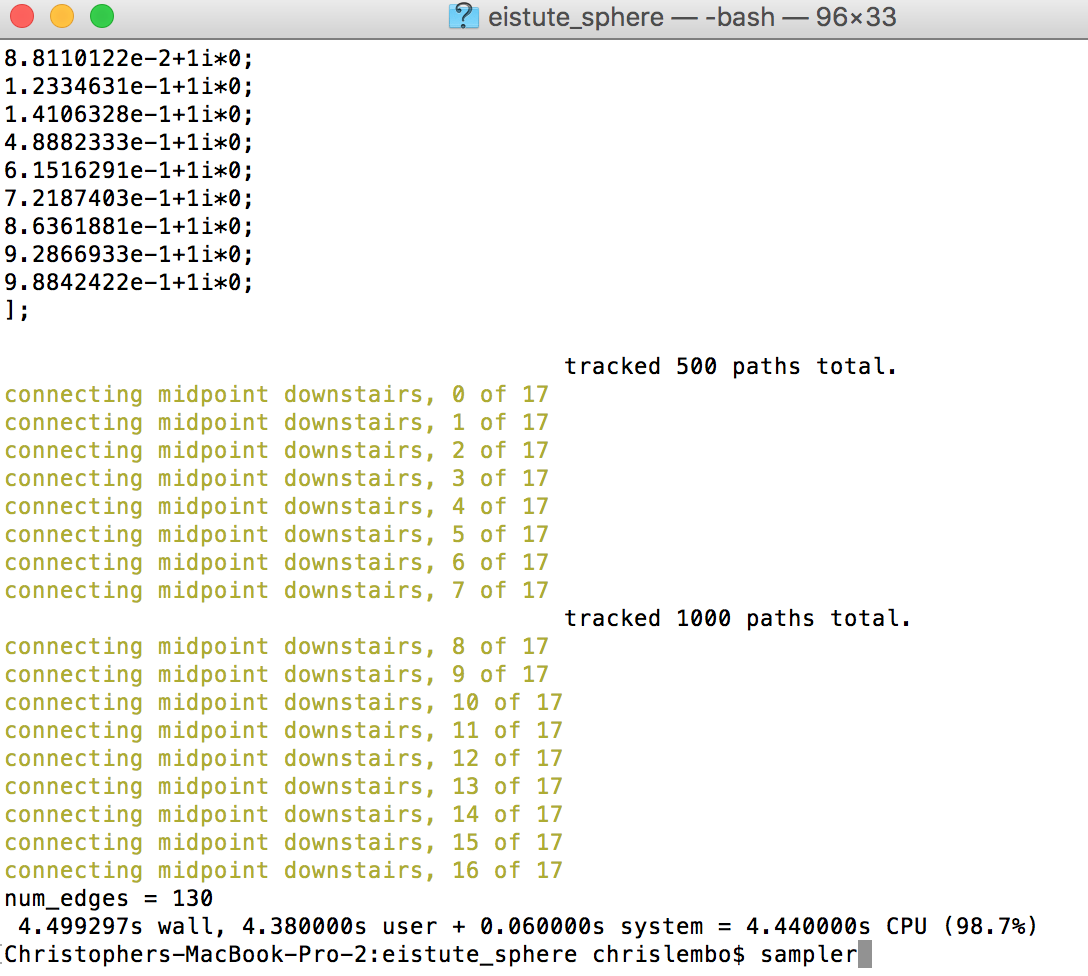
\includegraphics [width=0.4\textwidth]{curvesampler3} \\ \\ \\
\hline \\ 
Now use Matlab to produce the image of the curve
\begin{enumerate} 
	\item Go to the folder that holds your curve, then type 'gather\_br\_samples'
	\item To produce the image, type in 'bertini\_real\_plotter'
	\item you should end up with a figure along with matlab's display of viewing options
\end{enumerate}
& 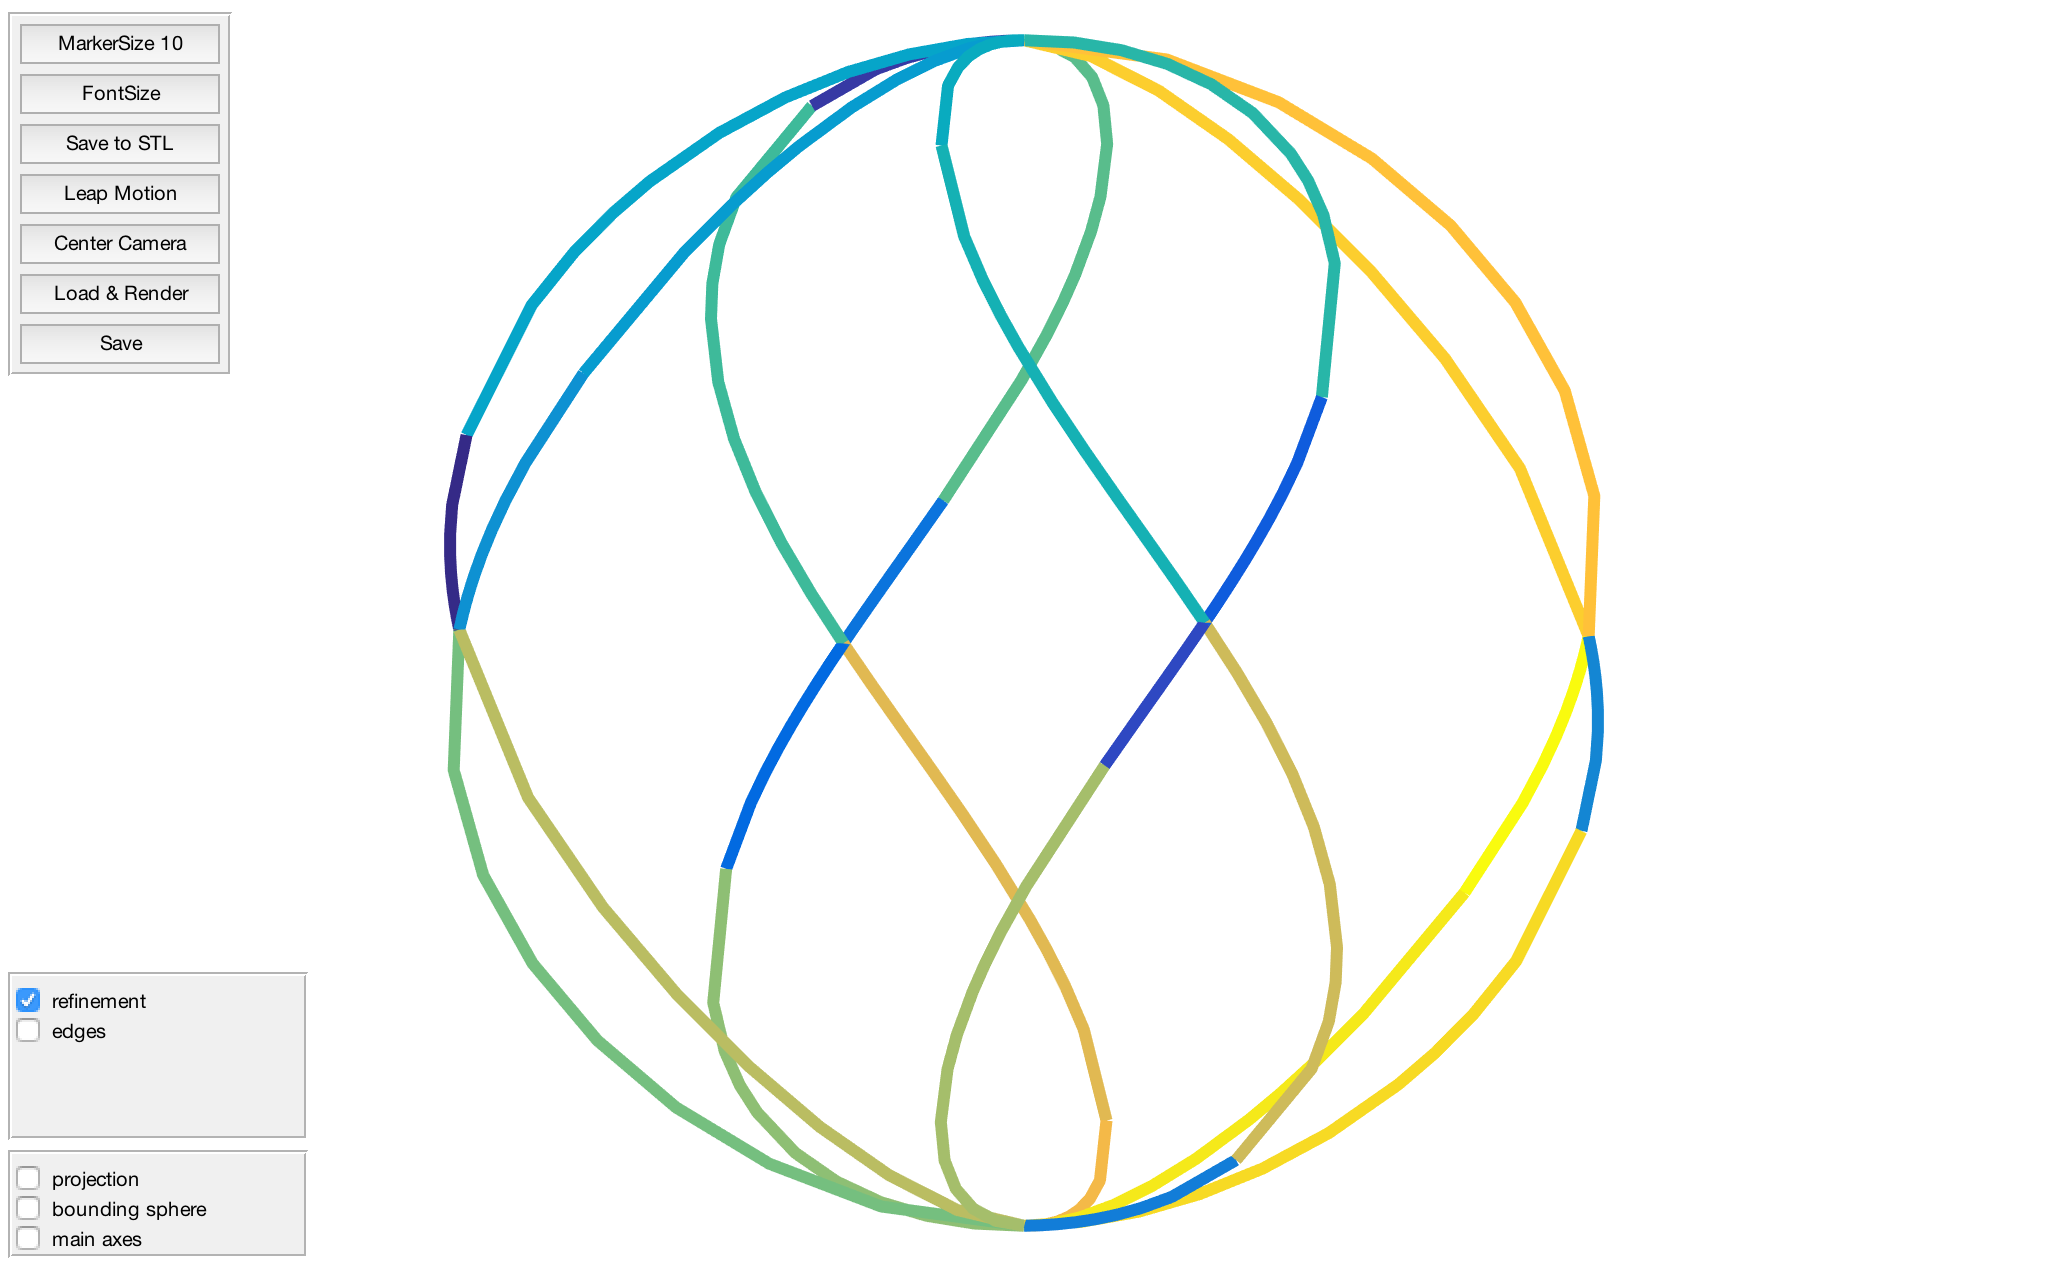
\includegraphics [width=0.4\textwidth]{curvesampler4.png} \\ \\ \\ 
  
\end{longtabu}


 	\subsubsection{Available curve sampling algorithms}
 	

 	There are three curve sampling algorithms available in the Sampler module for Bertini\_real.

 	\begin{enumerate}

 		\item {\tt -m a} -- Adaptive -- by movement of a predicted point.  Default choice.

 		\item {\tt -m d} -- Adaptive -- by distance between consective samples

 		\item {\tt -m f} -- Fixed -- every edge gets the same number of points

 	\end{enumerate}

The modes are accessed by calling sampler with the appropriate mode switch.


\paragraph{Curve sampling algorithm: Adaptive by movement}

This algorithm refines edge-by-edge until the predicted point, and the computed point, are close to each other.  It reduces sample density in regions of the curve which are flat, and has higher density in regions of high curvature.


\begin{figure}[H]
\begin{center}
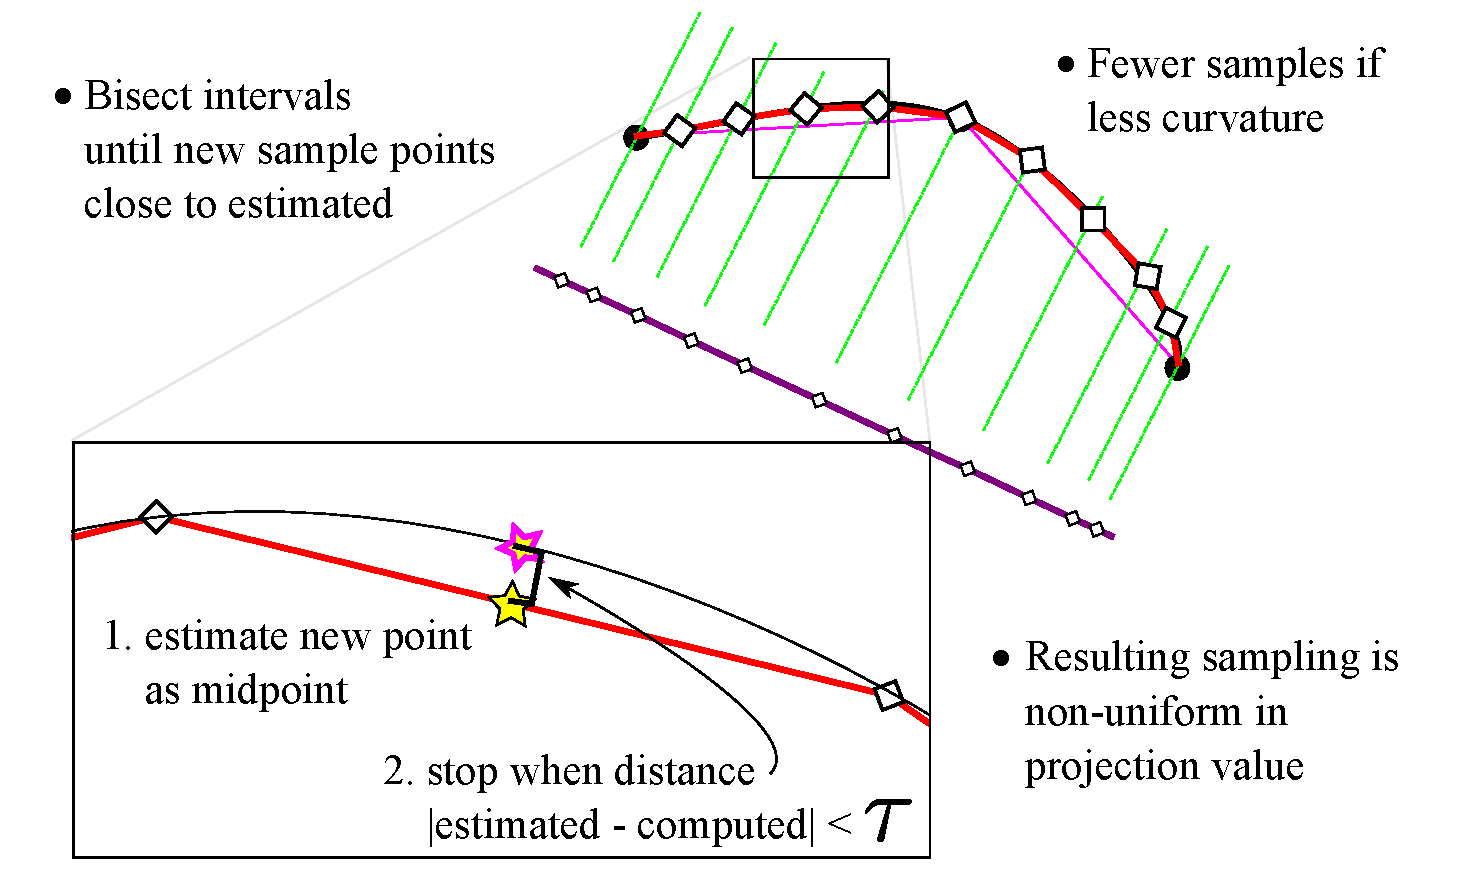
\includegraphics[scale = 0.4]{curve_sampling_adaptive_movement}
\caption[Adaptive-movement curve sampling]{Sampling a curve using movement-adaptive method.  New points are computed on the curve by bisecting intervals until the distance between the estimated midpoint and actual midpoint is less than convergence threshold $\tau$.}
\end{center}
\end{figure}
 
\begin{figure}[H]
\centering
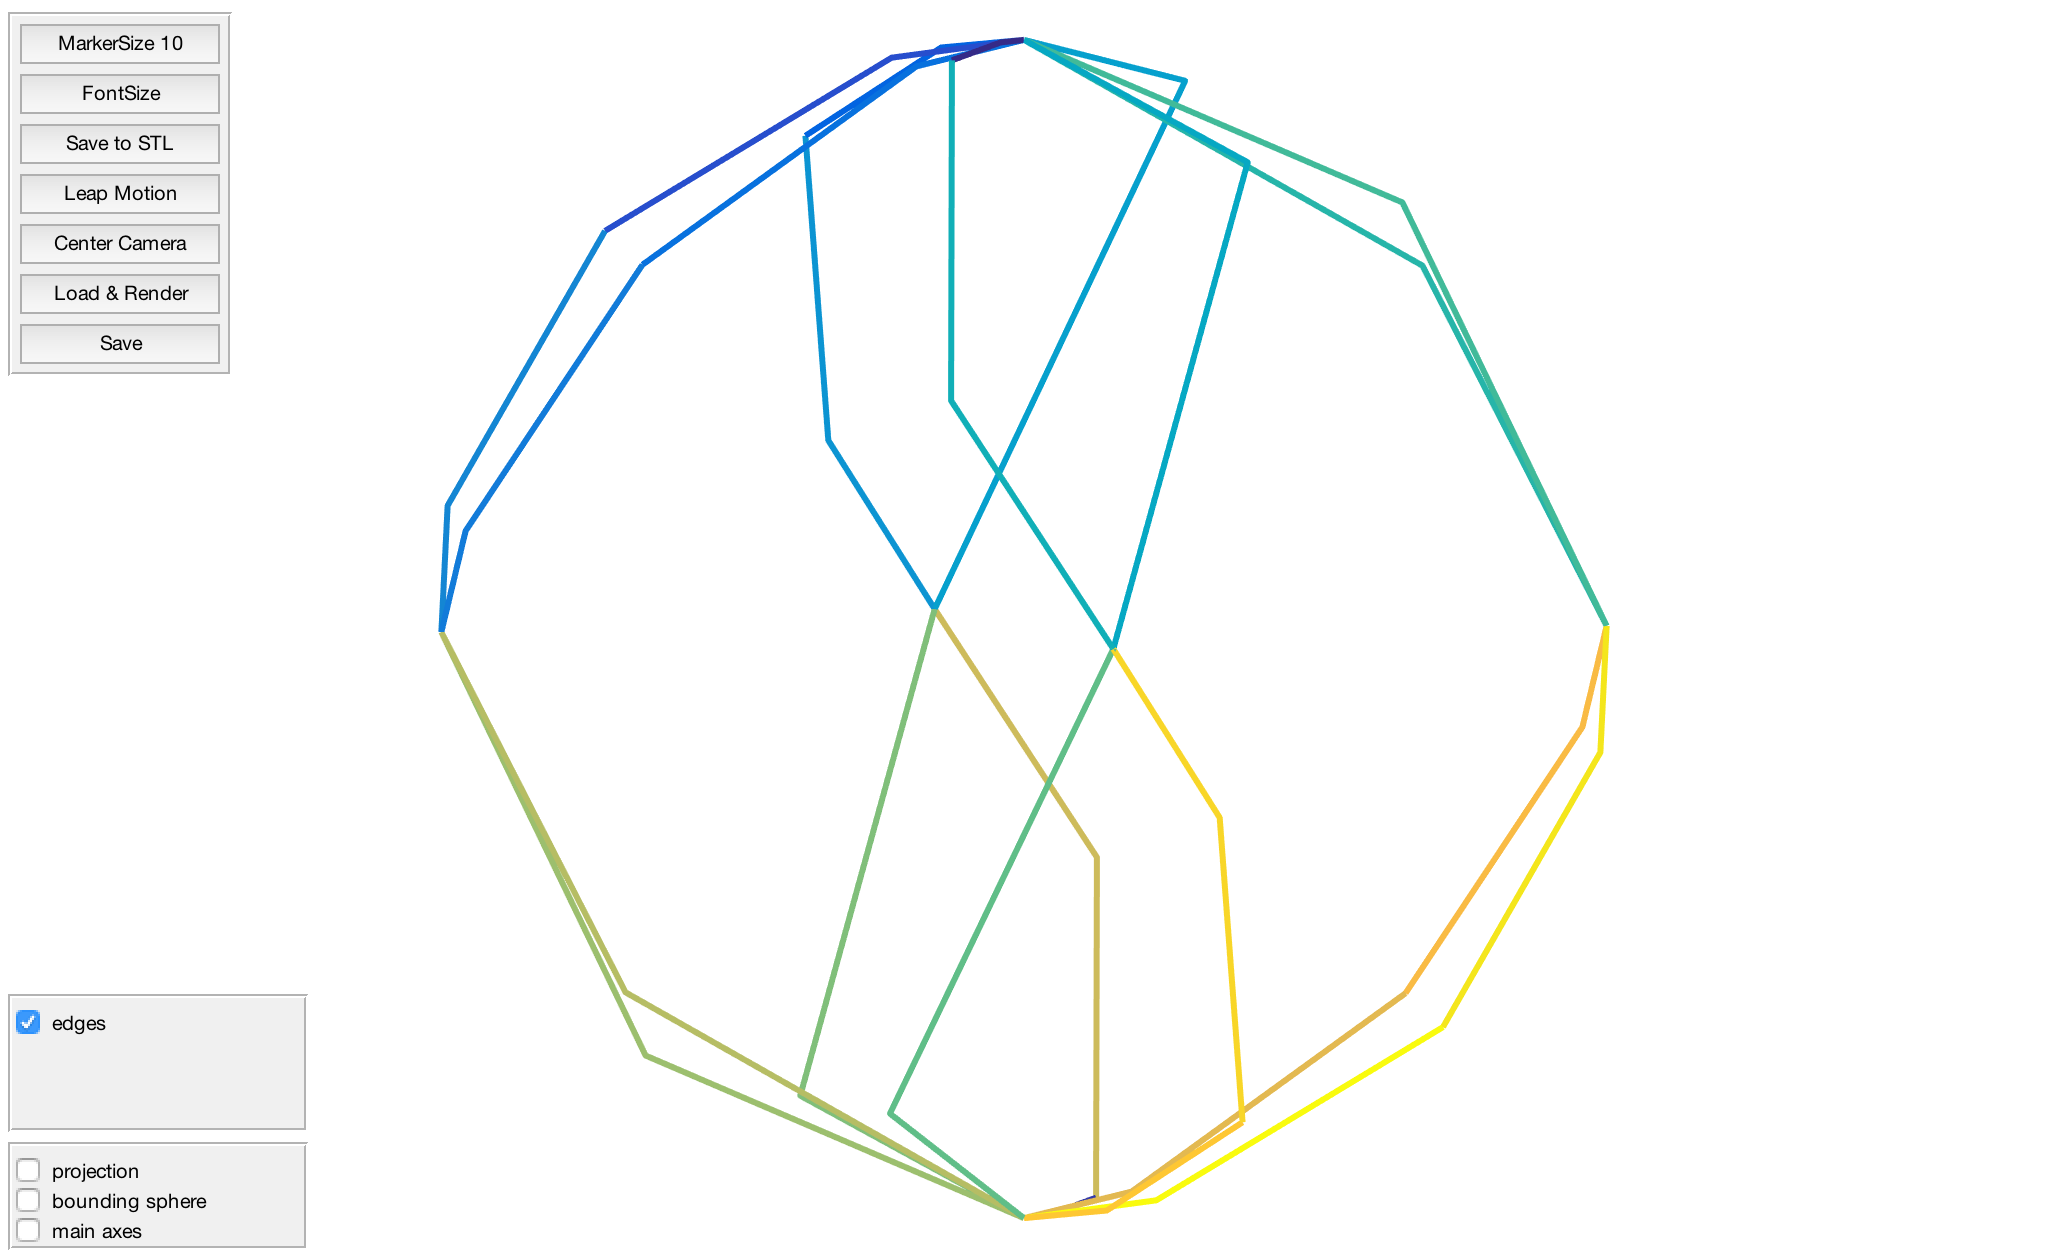
\includegraphics[width=0.5\textwidth]{curvesampler_adm.png}
\caption{This is an example of sampling a curve using the adaptive by movement mode. To replicate this, when invoking sampler, type in 'sampler -m a'}
\end{figure}

\paragraph{Curve sampling algorithm: Adaptive by distance}

The adaptive-by-distance refinement algorithm refines the edge by bisection until the distance between consecutive samples is less than some user-set threshold, or a maximum number of refinement iterations has been computed.  This algorithm works well, but over-samples flat regions of the curve, where relatively few points should be necessary.  


\begin{figure}[H]
\begin{center}
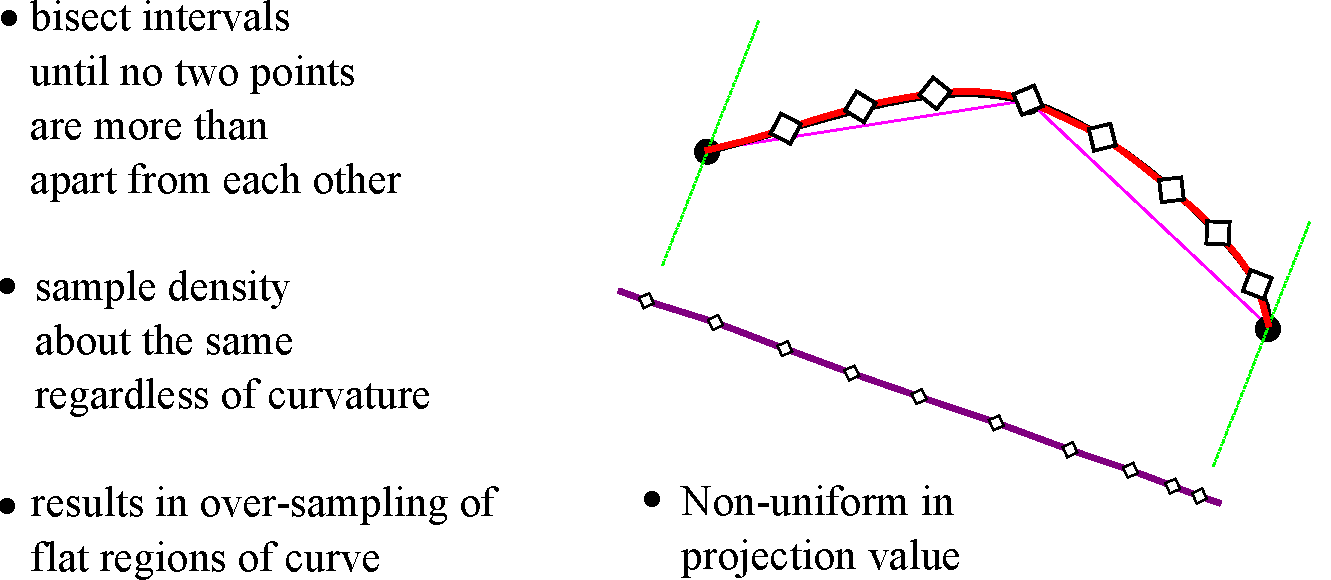
\includegraphics[scale = 0.4]{curve_sampling_adaptive_distance}
\caption[Adaptive-distance curve sampling]{Sampling a curve using distance-adaptive method.  New points are computed on the curve by bisecting intervals for which the distance between consecutive samples is larger than the convergence threshold $\tau$.}
\end{center}
\end{figure}

\begin{figure}[H]
\centering
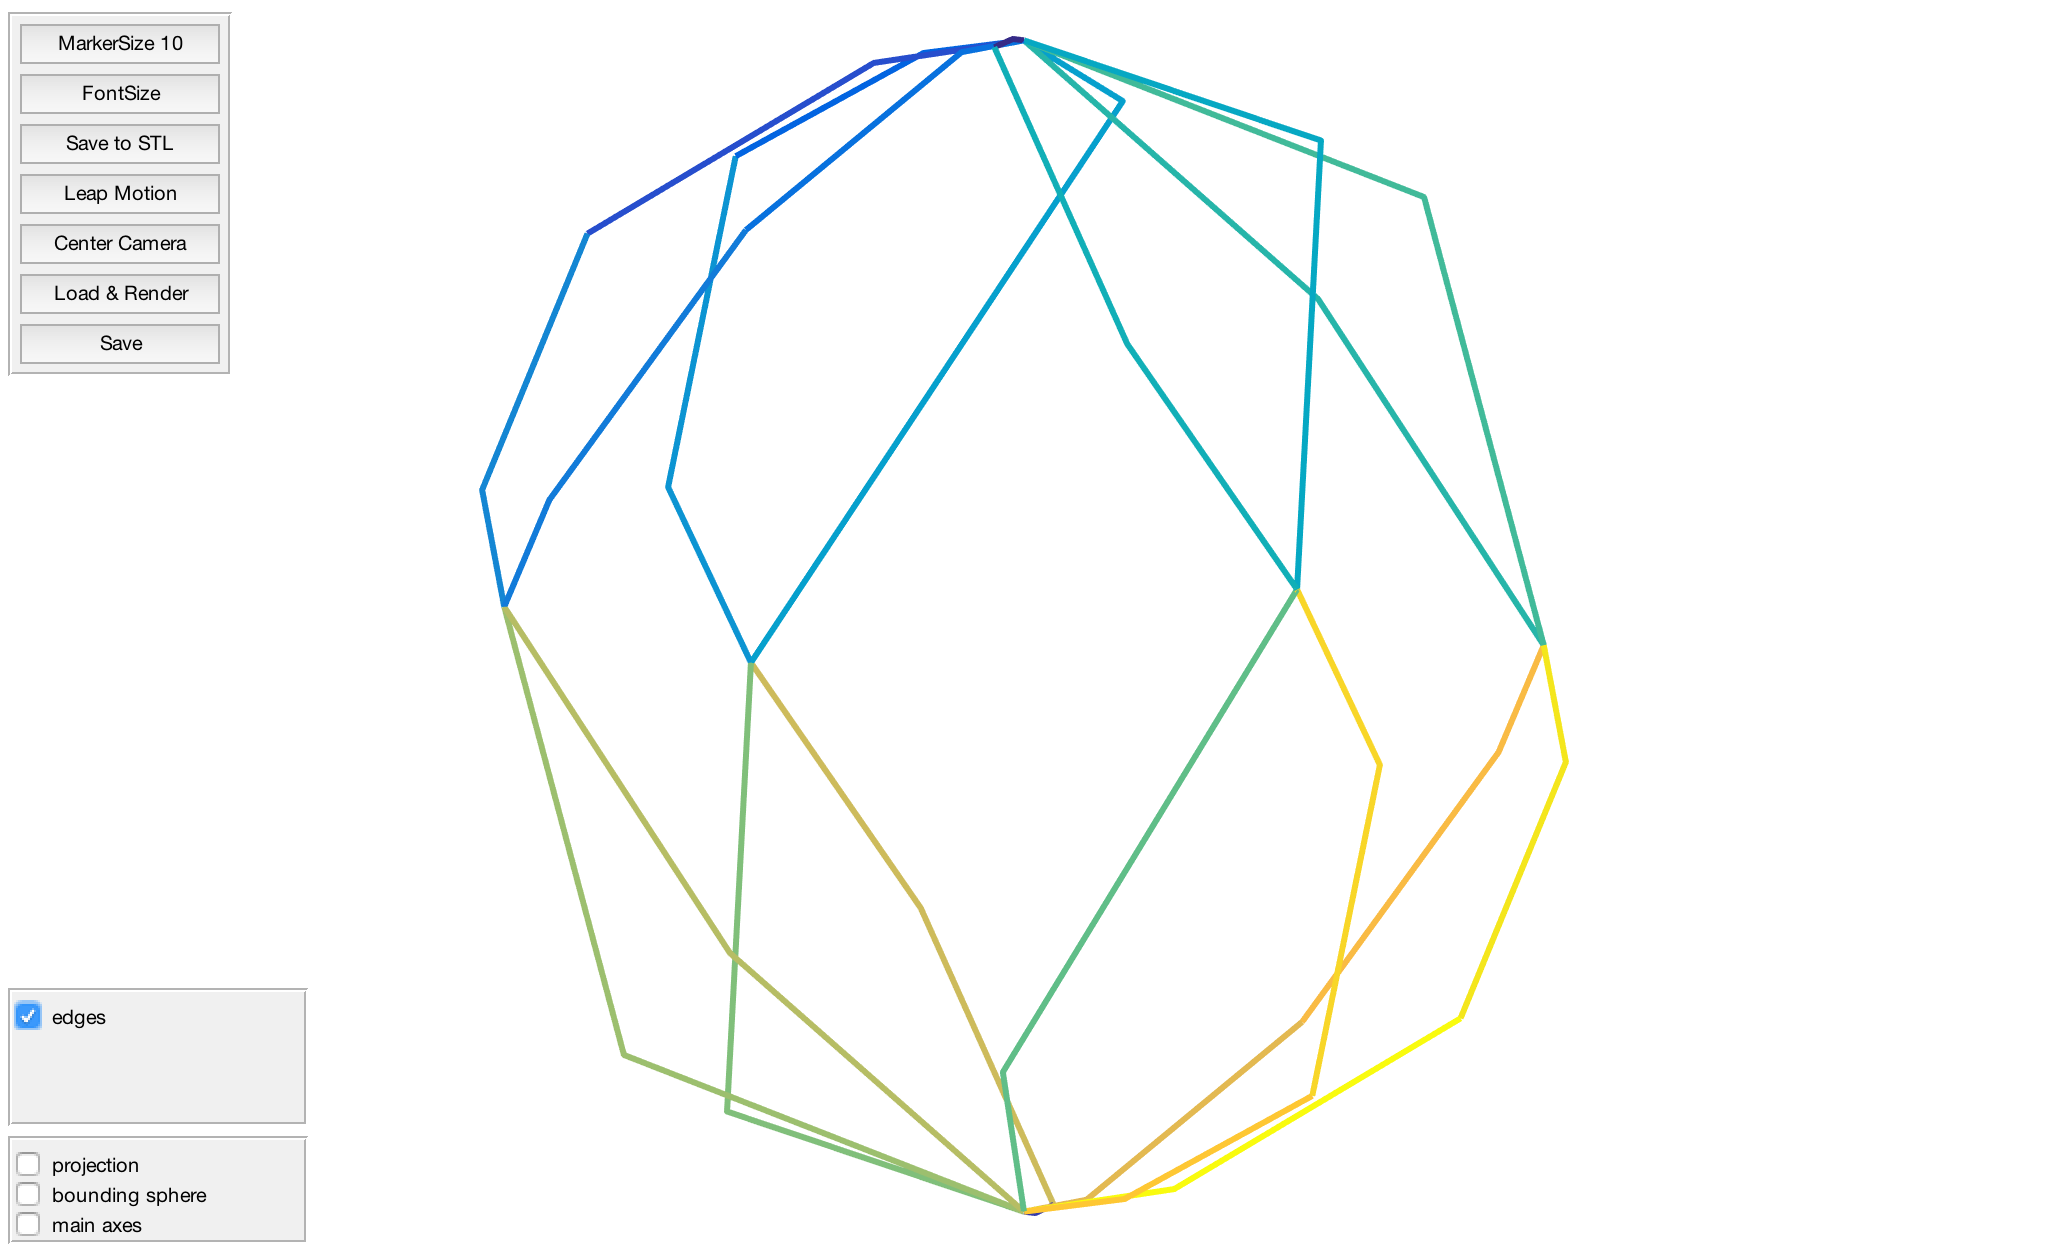
\includegraphics[width=0.5\textwidth]{curvesampler_add.png}
\caption{This is an example of sampling a curve using the adaptive by distance mode. To replicate this, when invoking sampler, type in 'sampler -m d'}
\end{figure}



\paragraph{Curve sampling algorithm: Fixed number}

This curve sampling algorithm produces a fixed (by the user) number of sample points per edge of the decomposed curve.  


\begin{figure}[H]
\begin{center}
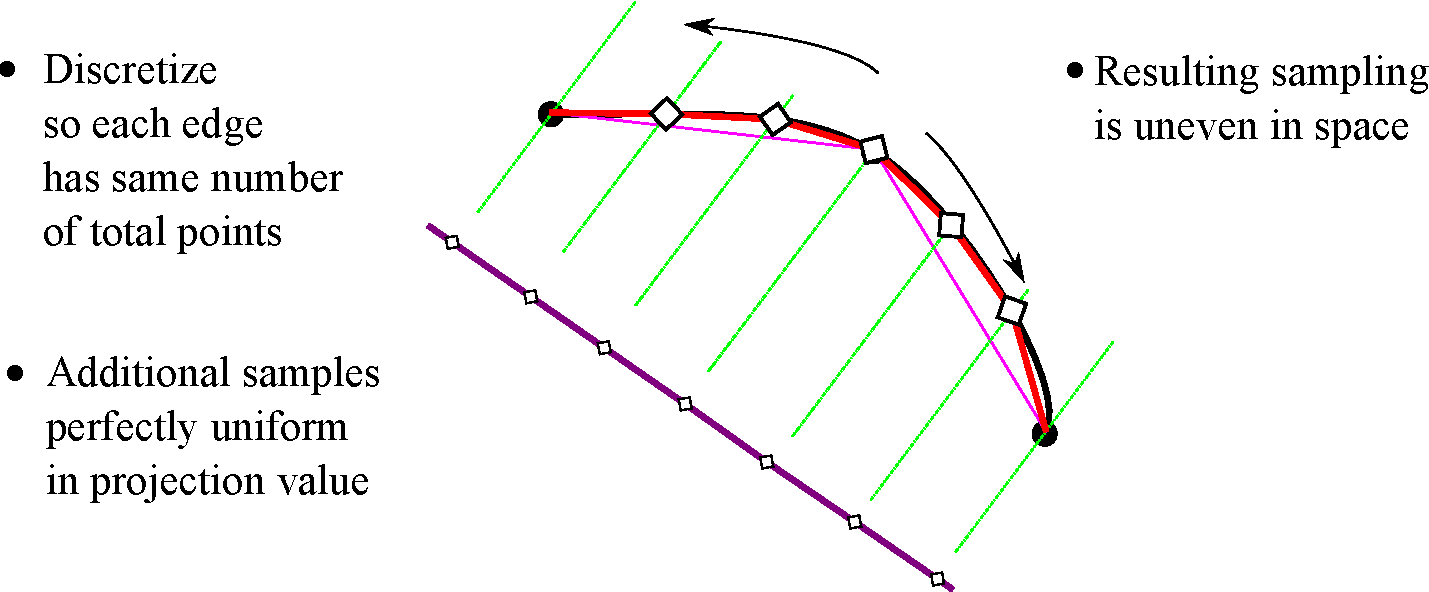
\includegraphics[scale = 0.4]{curve_sampling_fixed}
\caption[Fixed-number sampling of a curve -- how it works]{Fixed-number sampling of a curve.  The midpoint is homotoped so that a fixed number of sample points are computed on each edge of the curve.  The sample points are spaced uniformly in projection value, not in space.}
\end{center}
\end{figure}

\begin{figure}[H]
\centering
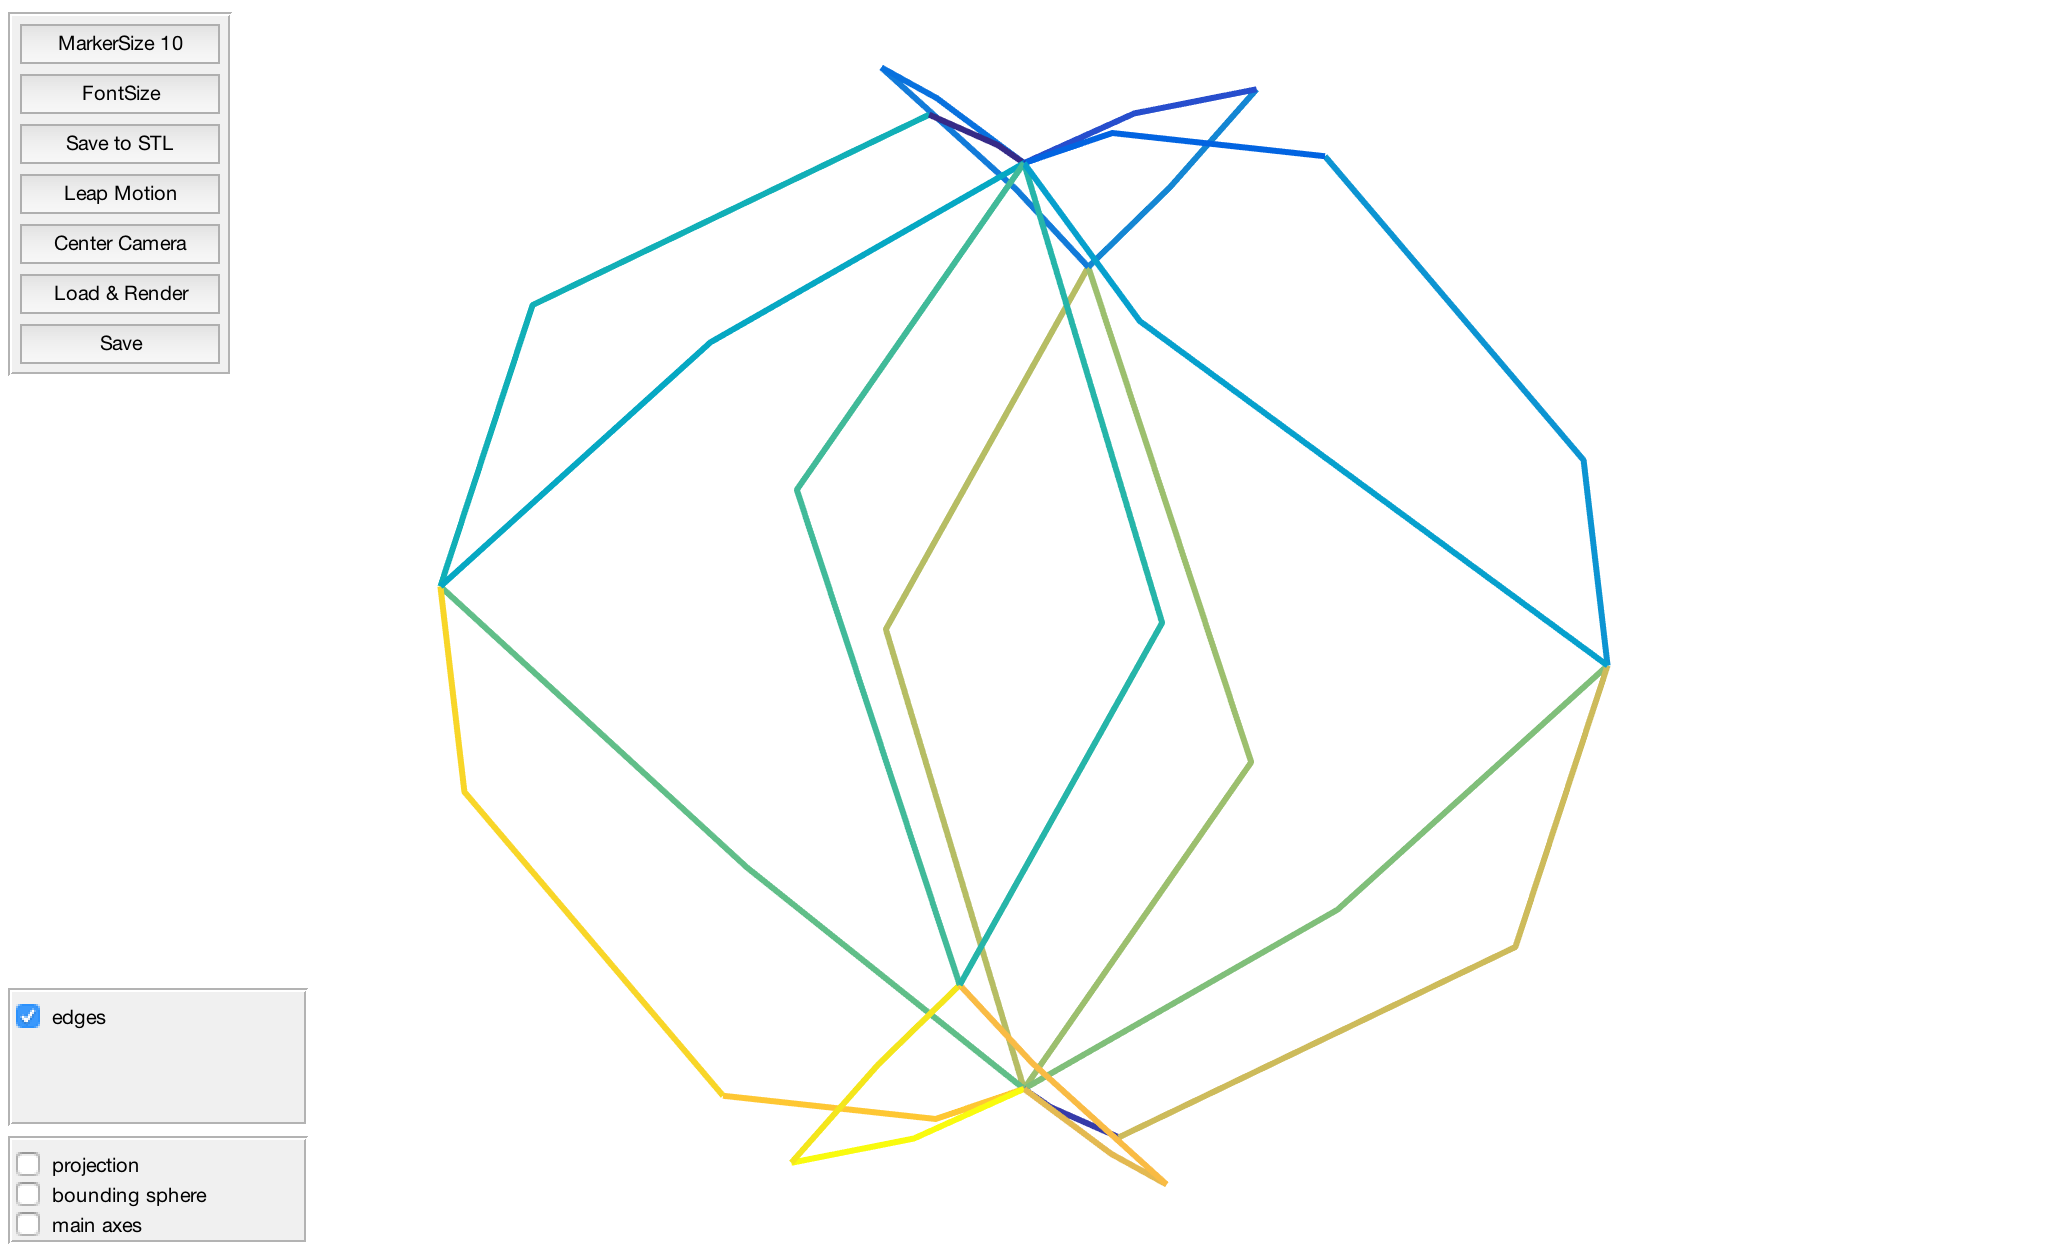
\includegraphics[width=0.5\textwidth]{curvesampler_f.png}
\caption{This is an example of sampling a curve using fixed mode. To replicate this, when invoking sampler, type in 'sampler -m f'}
\end{figure}

\subsection{Surfaces}

\subsubsection{Running Sampler (Using an Example)}

\subsubsection{Available surface sampling algorithms}






% EXTRA NOTES THAT I MIGHT USE(IGNORE THIS): Call \texttt{sampler} on the command line, e.g. \texttt{sampler -fixed 10} to sample each cell to have approximately $10^d$ samples on it, where $d$ is the dimension of the component. 




